


\usetikzlibrary{shapes} 

\ifnumequal{\value{rolldice}}{0}{
  \renewcommand{\va}{34}
  \renewcommand{\vb}{2}
  \renewcommand{\vc}{15}
  \renewcommand{\vd}{8}
  \renewcommand{\ve}{28}
}{
  \ifnumequal{\value{rolldice}}{1}{
    \renewcommand{\va}{40}
    \renewcommand{\vb}{1}
    \renewcommand{\vc}{12}
    \renewcommand{\vd}{9}
    \renewcommand{\ve}{31}
  }{
    \ifnumequal{\value{rolldice}}{2}{
      \renewcommand{\va}{36}
      \renewcommand{\vb}{2}
      \renewcommand{\vc}{13}
      \renewcommand{\vd}{8}
      \renewcommand{\ve}{29}
    }{
      \renewcommand{\va}{37}
      \renewcommand{\vb}{1}
      \renewcommand{\vc}{16}
      \renewcommand{\vd}{9}
      \renewcommand{\ve}{32}
    }
  }
}

\question The figure below shows a $B^{+}$ tree of degree $d=2$.
For simplicity, pointers in the leaf nodes are not shown. But remember that leaf 
nodes form a linked list. In the questions that follow, be mindful of overflow and underflow 
and maintain a fill-factor/occupancy of $\geq 50\%$. Root node can have $k$ keys where $1 \leq k \leq 2d$.


\watchout

  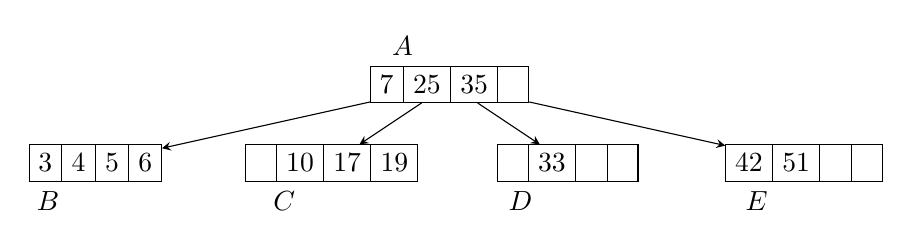
\begin{tikzpicture}[>= stealth, ->, level distance=10mm]
    \tikzstyle{bplus}=[rectangle split, rectangle split horizontal, draw]
    \tikzstyle{every node}=[bplus]
    \tikzstyle{level 1}=[sibling distance=30mm]
    \node[label=90:$A$]{7\nodepart{two} 25\nodepart{three} 35}
      child {node[label=270:$B$] {3 \nodepart{two} 4\nodepart{three} 5\nodepart{four} 6}}
      child {node[label=270:$C$] {\vd\nodepart{two} 10\nodepart{three} 17\nodepart{four} 19}}
      child {node[label=270:$D$] {\ve\nodepart{two} 33}}
      child {node[label=270:$E$] {42 \nodepart{two} 51}} ;
  \end{tikzpicture}

\begin{parts}
  \part[2] What will the $B^{+}$ tree look like after inserting $\mathbf{\va, \vb}$ and $\mathbf\vc$ - in that order?

\begin{solution}[\halfpage]
    \begin{align}
      &D+\va\longrightarrow\text{ no problem } \\
      &\underbrace{B+\vb}_{\texttt{overflow}} \longrightarrow \underbrace{(B_1, B_2)}_{\texttt{split}} 
      + \underbrace{(A+4)}_{\texttt{4 added to A}} \\
      &\underbrace{C + \vc}_{\texttt{overflow}}\longrightarrow
      \underbrace{(C_1, C_2)}_{\texttt{split}} + \underbrace{(A+\vc)}_{\texttt{overflow}}\longrightarrow
      \underbrace{(C_1, C_2)}_{\texttt{split}} + \underbrace{A\longrightarrow(A_1, A_2, A_3)}_{\texttt{split}}
    \end{align}
  \end{solution}
  \begin{tikzpicture}[>= stealth, ->, level distance=10mm]
    \tikzstyle{bplus}=[rectangle split, rectangle split horizontal, rectangle split ignore empty parts, draw]
    \tikzstyle{every node}=[bplus]
    \tikzstyle{level 1}=[sibling distance=70mm]
    \tikzstyle{level 2}=[sibling distance=20mm]
    \node[label=90:$A_1$]{\vc}
      child {node[label=180:$A_2$] {4\nodepart{two} 7}
        child {node[label=270:$B_1$] {\vb\nodepart{two} 3}}
        child {node[label=270:$B_2$] {5\nodepart{two} 6}}
        child {node[label=270:$C_1$] {\vd\nodepart{two} 10}}
      }
      child {node[label=180:$A_3$] {25\nodepart{two} 35}
        child {node[label=270:$C_2$] {17\nodepart{two} 19}}
        child {node[label=270:$D$] {\ve\nodepart{two} 33\nodepart{three} \va}}
        child {node[label=270:$E$] {42 \nodepart{two} 51}}
      };
  \end{tikzpicture}

  \part[2] If $\mathbf{\ve}$ and $\mathbf{\vd}$ are now removed from the tree - in that order - 
  \textbf{after} the insertions done in part (a), then what will the $B^{+}$ tree look like?

\begin{solution}[\halfpage]
    \begin{align}
      &D-\ve\longrightarrow\text{ no problem } \\
      &\underbrace{C_1-\vd}_{\texttt{underflow}}\longrightarrow(B_2+C_1) + \text{ move 7 to }A_2 \text{ and copy 4 to }B_2
    \end{align}
  \end{solution}
  \begin{tikzpicture}[>= stealth, ->, level distance=10mm]
    \tikzstyle{bplus}=[rectangle split, rectangle split horizontal, rectangle split ignore empty parts, draw]
    \tikzstyle{every node}=[bplus]
    \tikzstyle{level 1}=[sibling distance=70mm]
    \tikzstyle{level 2}=[sibling distance=20mm]
    \node[label=90:$A_1$]{\vc}
      child {node[label=180:$A_2$] {4\nodepart{two} 6}
        child {node[label=270:$B_1$] {\vb\nodepart{two} 3}}
        child {node[label=270:$B_2$] {4\nodepart{two} 5}}
        child {node[label=270:$C_1$] {7\nodepart{two} 10}}
      }
      child {node[label=180:$A_3$] {25\nodepart{two} 35}
        child {node[label=270:$C_2$] {17\nodepart{two} 19}}
        child {node[label=270:$D$] {33\nodepart{two} \va}}
        child {node[label=270:$E$] {42 \nodepart{two} 51}}
      };
  \end{tikzpicture}

\end{parts}

\ifprintanswers\begin{codex}\end{codex}\fi
